\section{untrip - WIP}
Sloppily coped from\\ \verb|MT-Tech-SETO\researchDocs\TEX\one-offs\200901-refinedUntripResults2|

Variables to note in associated examples (where \verb|x| is the internal model number):
\begin{itemize}
\item exciter $V_{ref} = $ \verb|g.exc.exc_pot(x,3)|
\item governor $P_{ref} = $ \verb|g.tg.tg_pot(x,5)|
\item governor $\omega_{ref} = $ \verb|g.tg.tg_con(x,3)|
\end{itemize}


\textbf{Test System}\ A simple 3 machine system was used for `un-trip' testing.
All machines were modeled with governors, exciters, and PSS.
Most model parameters are the same, with the exception of MVA base.
Generators 1, 2, and 3, have an $M_{base}$ of 500, 200, and 100 MVA respectively. \\
The experimental goal was to trip Generator 3 off-line, and then `nicely' re-connect it.\\

This is different from the previous test in that ramps of $P_{ref}$ and $\omega_{ref}$ happen concurrently, an extra initialization of the governor was removed, and instead of using \verb|tg_sig| to restore governor $P_{ref}$, the value is ramped directly.

\begin{center}
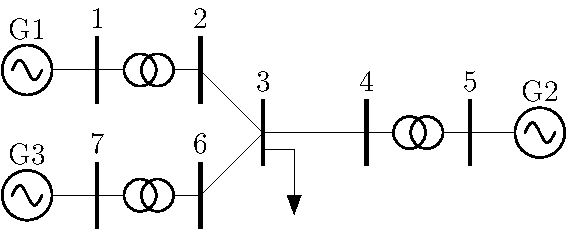
\includegraphics[width=.6\linewidth]{examples/untrip/200831-3mach7bus}
\end{center}

\textbf{Test Event Time Line:}
\begin{itemize}
\itemsep 0 em
\item $t=0$ - System initialized
\item $t=5$ - Generator 3 trips off.
Associated derivatives, $P_{mech}$, and governor $P_{ref}$ set to zero.
\item $t=15$ - Generator 3 re-synced to system and infinite reactance reset to original value. 

\item $t=20-25$ - The governor attached to Generator 3 is reinitialized and the $\omega_{ref}$ value is ramped to its original value. 
This causes mechanical power to be generated by Generator 3 which causes minor transients in system machine speed.
\item $t=35$ - The exciter and PSS on generator 3 is re-initialized and the exciter bypass is removed.
%This causes more reactive power flow into generator 3, the attached bus voltages to decrease, and system speed to increase. 
\item $t=45-65$ - Ramping the governor $P_{ref}$ to the original value increases system speed  and real power flow from Generator 3 while the ramping of exciter reference voltage to its original value decreases system speed and increases reactive power flow from generator 3.
\item $t=150$ - Simulation End
\end{itemize}

\textbf{Observations of Note:}
\begin{itemize}
\itemsep 0 em
%\item The re-connected speed of Generator 3 was set to match Generator 1.
%\item The ramping of R causes a minor 
%\item The exciter was not being initialized to the correct reference voltage time index (i.e. \verb|g.exc.exc_pot(x,3)| referenced index 1 instead of $k$ ). This has been resolved however the exciter still produces a transient when it is bypassed.
\item Nicely `un-tripping' a generator seems possible.
%\item Generator 3 power returns $P_{ref}$ value of 0.5 PU.
\item System appears to return to original state.
%\item Exciter transient caused by bypass removal seems tricky to avoid.\\
%Should probably be reinitialized and enabled at the same time as generator un-trip.
\item Scenario development using FTS as VTS will likely present additional reinitialization issues.
\end{itemize}

\pagebreak
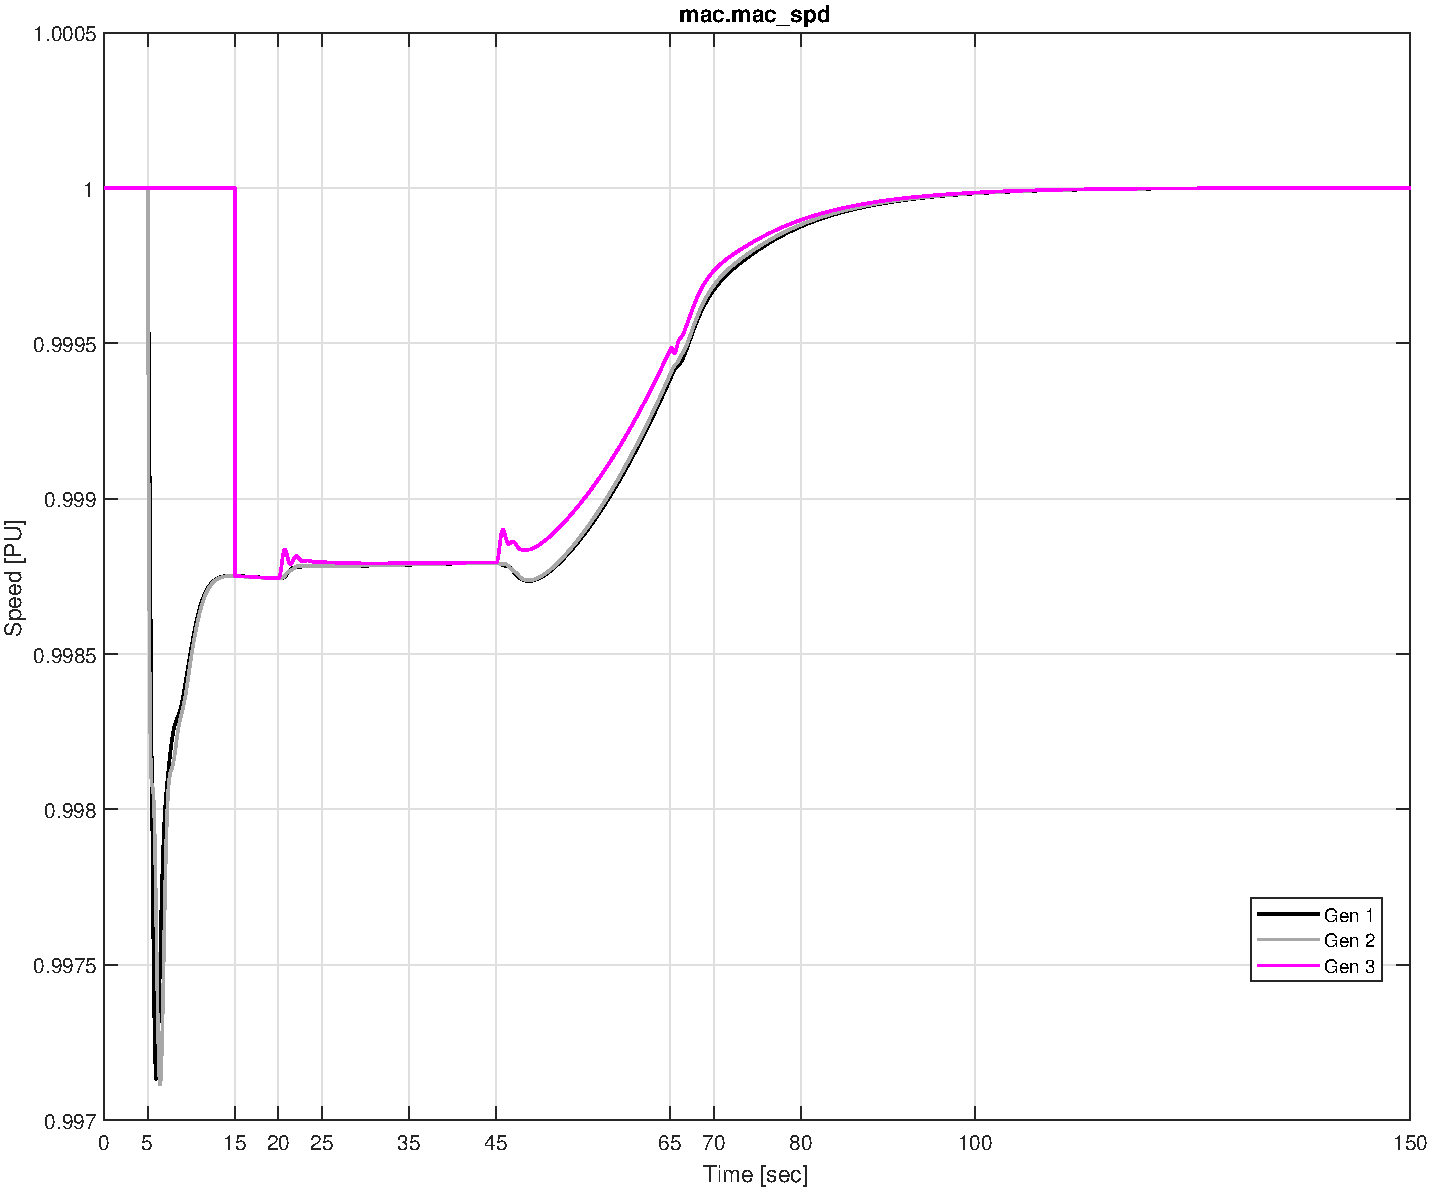
\includegraphics[width=\linewidth]{examples/untrip/combinedSpeed}
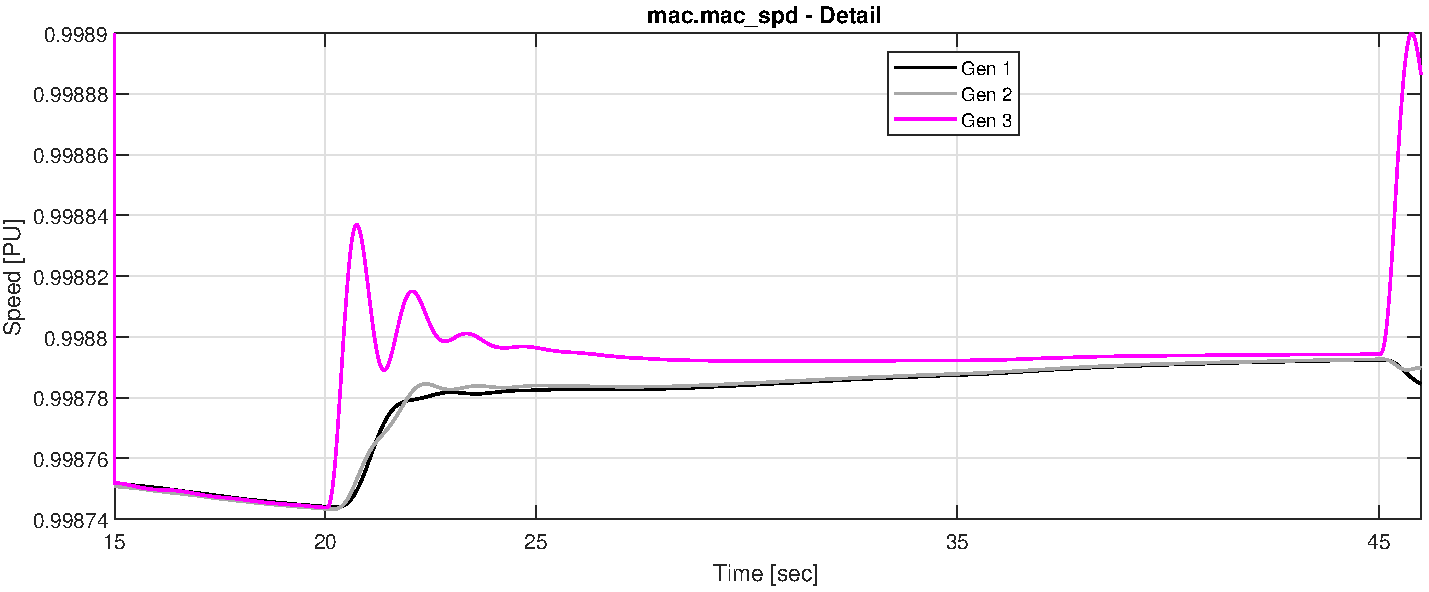
\includegraphics[width=\linewidth]{examples/untrip/combinedSpeedDetail}


\pagebreak
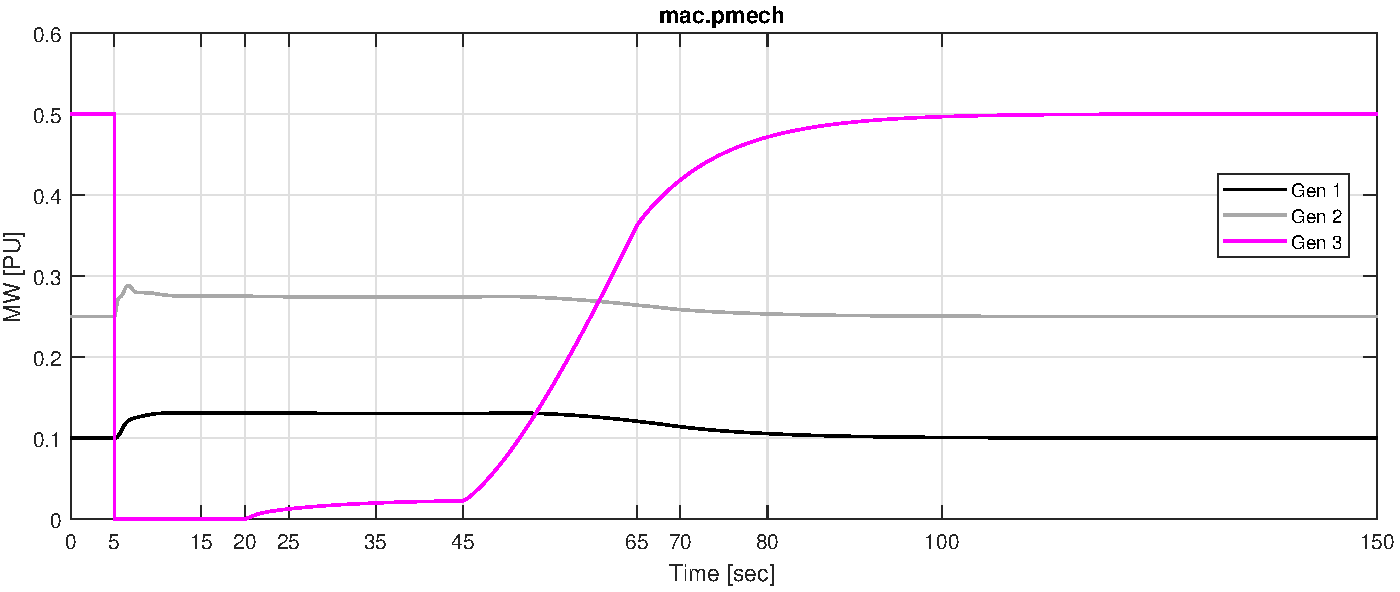
\includegraphics[width=\linewidth]{examples/untrip/combinedPmech}
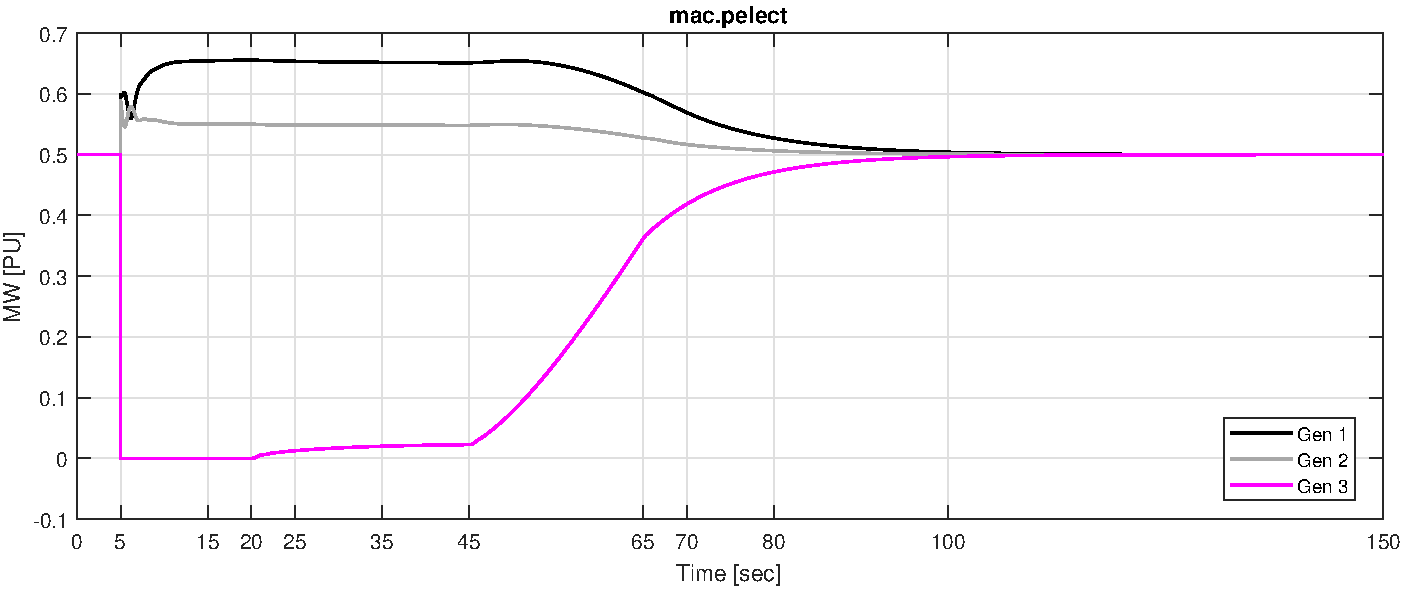
\includegraphics[width=\linewidth]{examples/untrip/combinedPelect}
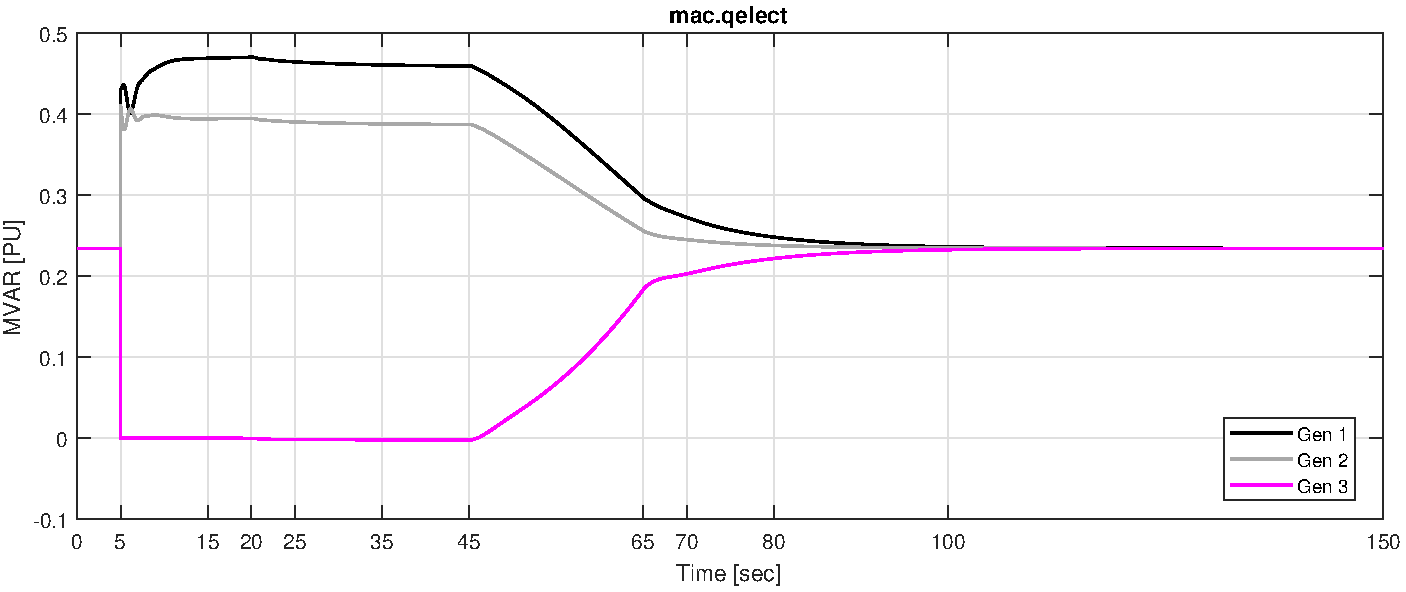
\includegraphics[width=\linewidth]{examples/untrip/combinedQelect}

\pagebreak
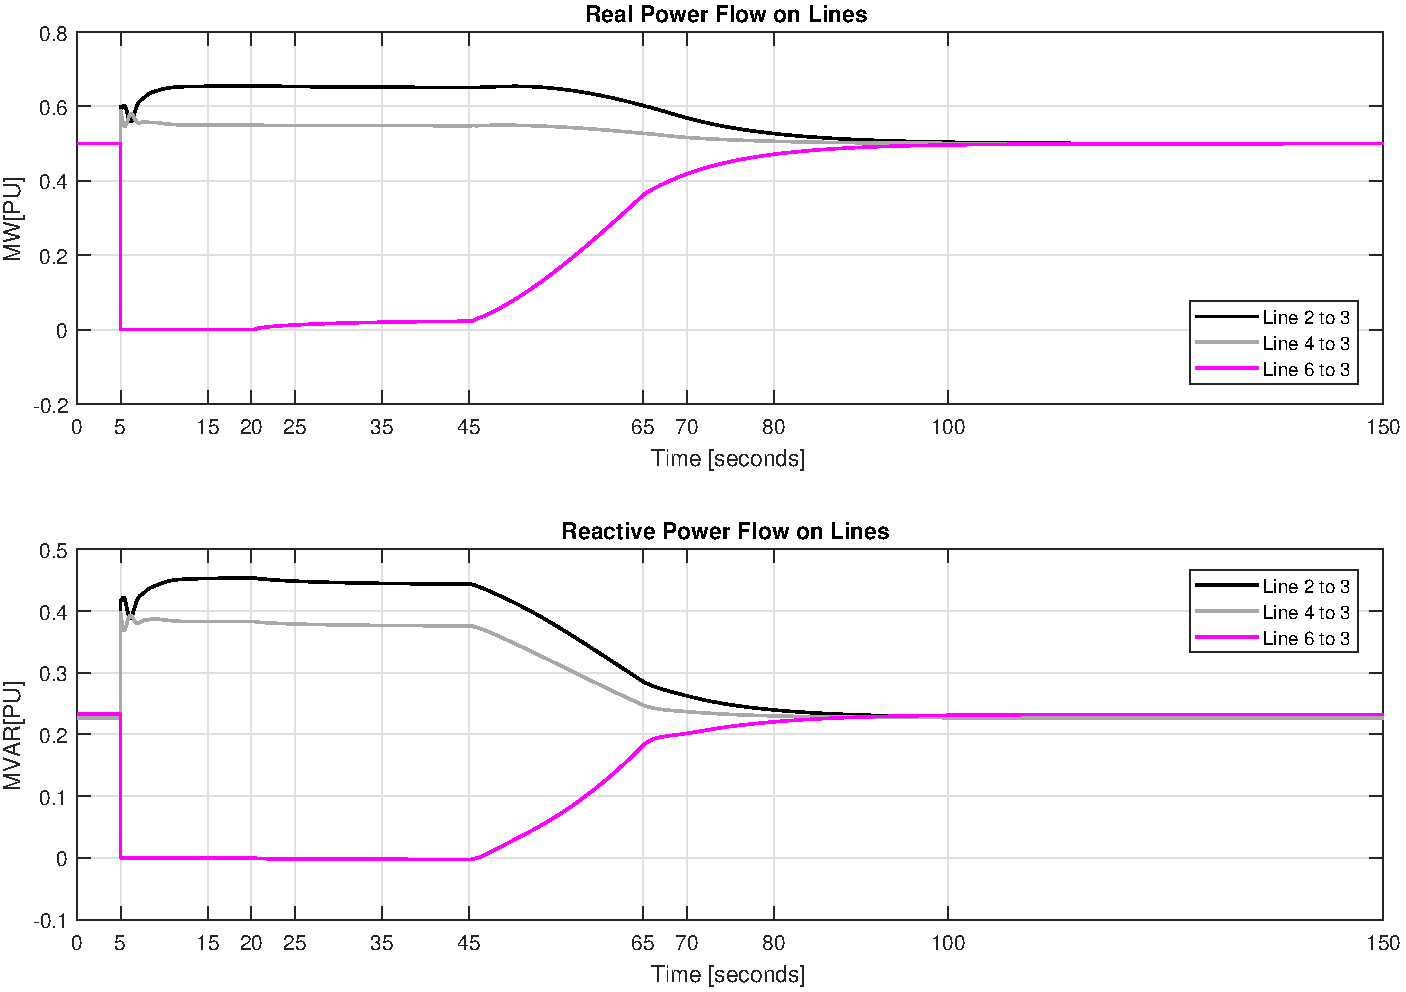
\includegraphics[width=\linewidth]{examples/untrip/combinedLoadFlow}
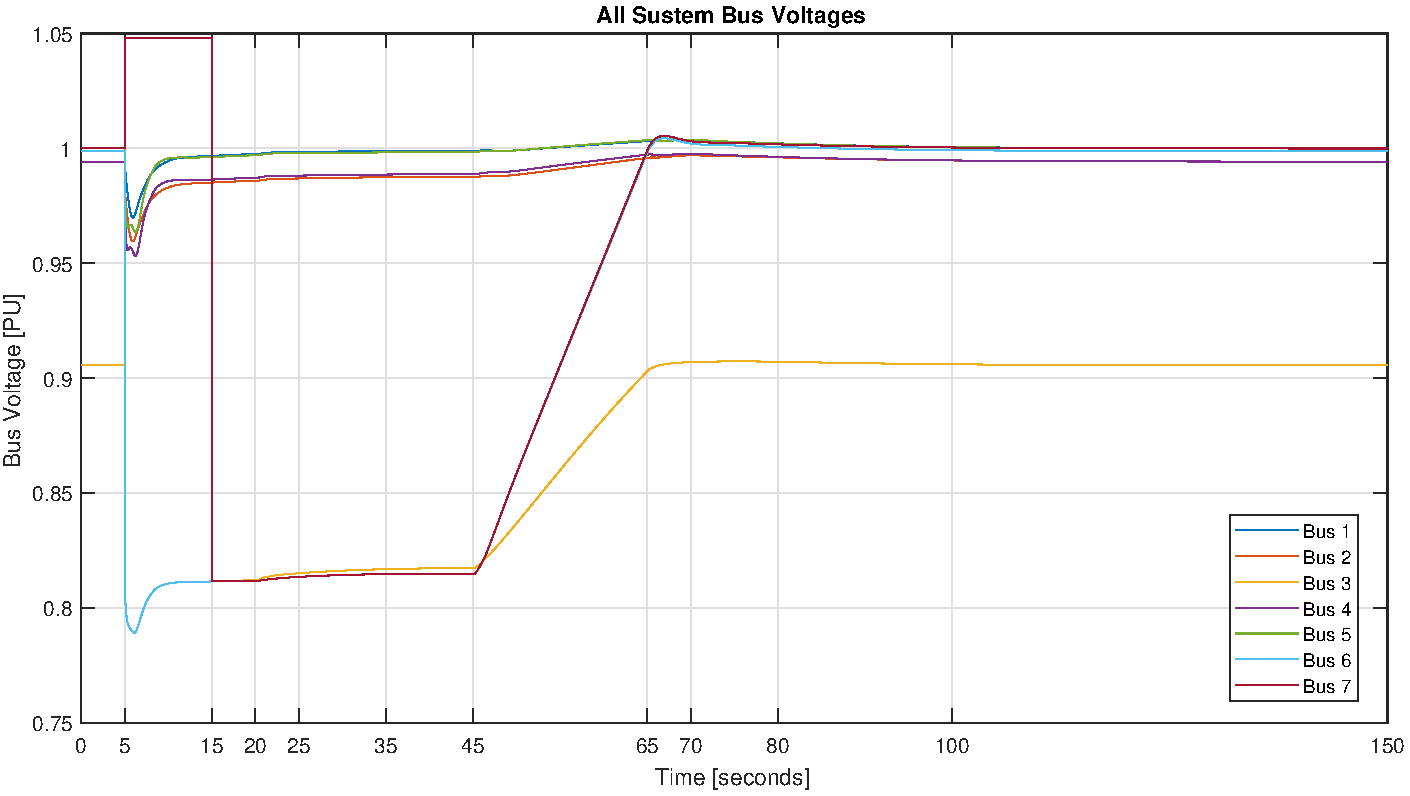
\includegraphics[width=\linewidth]{examples/untrip/combinedBusV}


\pagebreak
\textbf{Machine Trip Logic Code} \ \\
Most `un-trip' action takes place in the \verb|mac_trip_logic| file.
Such actions include:
\begin{itemize}
\item Trip generator 3
\item Set mechanical power to zero and bypass governor
\item Bypass exciter
\item Un-trip generator 3
\item Re-initialize machine
\item Re-init governor
\item Ramp governor $\omega_{ref}$
\item Re-init and remove bypass on exciter and PSS
\item Ramp exciter reference
\end{itemize} 

It should be noted that the \verb|mac_trip_logic| routine usage was created `pre-global g', and as a result, passes variables in and out that are essentially globals.
Realistically, only a data index would need to be passed into the function, and any action can take place directly on the associated \verb|g.mac.mac_trip_states| vector or other required global.

\inputminted[
		frame=lines,
		framesep=2mm,
		baselinestretch=1.2,
		bgcolor=gray!13,
		fontsize=\footnotesize,
		linenos,
		breaklines
		]{MATLAB}% lang
		{../../../../PST/0-examples/unTrip/mac_trip_logic_Gen_3_G2.m}% file name

\pagebreak
\textbf{Turbine Governor Modulation Code} \ \\
The \verb|mtg_sig| file was used to ramp the governors $P_{ref}$ back to the original value.
\inputminted[
		frame=lines,
		framesep=2mm,
		baselinestretch=1.2,
		bgcolor=gray!13,
		fontsize=\footnotesize,
		linenos,
		breaklines
		]{MATLAB}% lang
		{../../../../PST/0-examples/unTrip/mtg_sig_PrefRamp.m}% file name
		